\paragraph{Fake Rate Determination (OS method)}
In order to measure the lepton fake ratios $f_{e}$ and $f_{\mu}$, we select samples of $Z(\ell\ell)+e$ and $Z(\ell\ell)+\mu$ events that are expected to be completely dominated by final states which include a $Z$ boson and a fake lepton. 
These events are required to have two same flavour, opposite charge leptons with $p_{T} > 20/10$~GeV passing the tight selection criteria, thus forming the $Z$ candidate. In addition, there is exactly one lepton passing the loose selection criteria as defined above. 
This lepton is used as the probe lepton for the fake ratio measurement. The invariant mass of this lepton and the opposite sign lepton from the reconstructed $Z$ candidate should satisfy $m_{2l} > 4$~GeV. 


The fake ratios are evaluated using the tight requirement 
$|M_{inv}(\ell_{1},\ell_{2}) - M_{Z}| < 7 $~GeV, to reduce the 
contribution from photon (asymmetric) conversions populating low masses. 
The fake ratios are measured in bins of the transverse momentum of the loose lepton in the barrel and endcap regions. 
The electron and muon fake rates are measured within 
$|M_{inv}(\ell_{1},\ell_{2}) - M_{Z}| < 7 $~GeV and $E_{\mathrm{T}}^\text{miss}  < $ 25~GeV, 
separately for the 2016, 2017 and 2018 data, and are shown in Figure~\ref{fig:os_fakerates}. 


\paragraph{Fake Rate Application (OS method)}
\label{sec:zxA}

Two control samples are obtained as subsets of the four lepton events
which pass the first step of the selection ({\it First Z} step, see
section~\ref{sec:zzcandsel}), requiring an additional pair of identified
loose leptons of same flavour 
and opposite charge, that pass the ${\rm SIP_{3D}}$, dxy and dz cuts. 
The events must satisfy all kinematic cuts applied for the {\it Higgs phase space} selection
(see~\ref{sec:zzcandsel}).

The first control sample is obtained by
requiring that the two loose leptons, which do not make the $Z_1$ candidate, 
do not pass the final selection criteria, while the other two leptons pass
the final selection criteria by definition of the $Z_1$. 
This sample is denoted as ``2 Prompt + 2 Fail'' ({\it 2P+2F}) sample. 
It is expected to be populated with events that intrinsically have only two prompt leptons 
(mostly $DY$, with a small fraction of $t \bar{t}$ and $Z \gamma$ events).
The second control sample is obtained by requiring one of
the four leptons not to pass the final identification criteria 
and selection cuts on SIP, dxy and dz and is denoted as ``3 Prompt + 1 Fail'' ({\it 3P+1F}) sample. 
%======= 
\begin{figure}[!]
\begin{center}
    {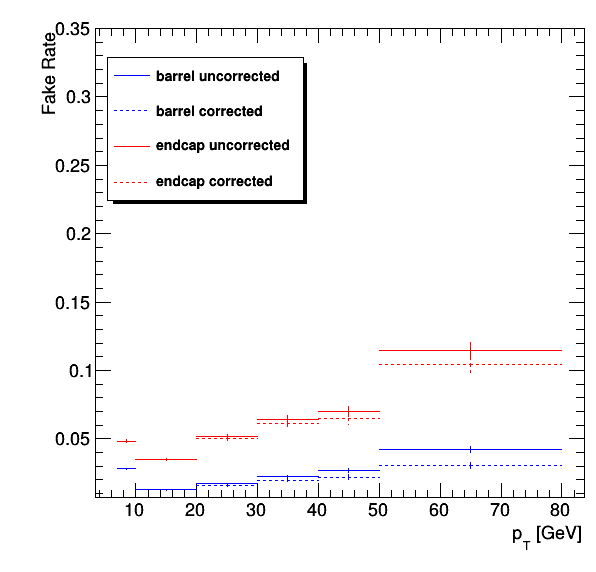
\includegraphics [width=0.45\textwidth] {Figures/RedBkg/FR/FR_OS_electrons_2016.png}}
    {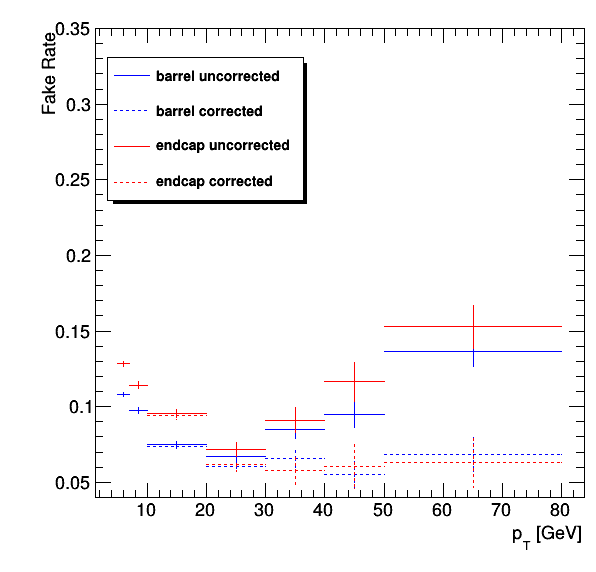
\includegraphics [width=0.45\textwidth] {Figures/RedBkg/FR/FR_OS_muons_2016.png}} \\
    {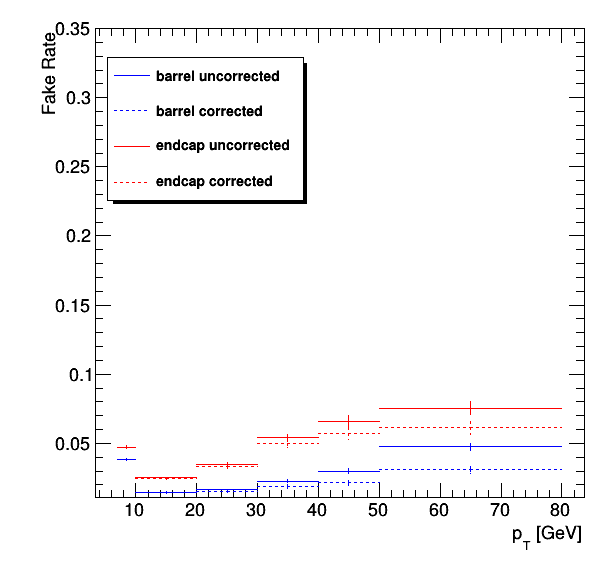
\includegraphics [width=0.45\textwidth] {Figures/RedBkg/FR/FR_OS_electrons_2017.png}}
    {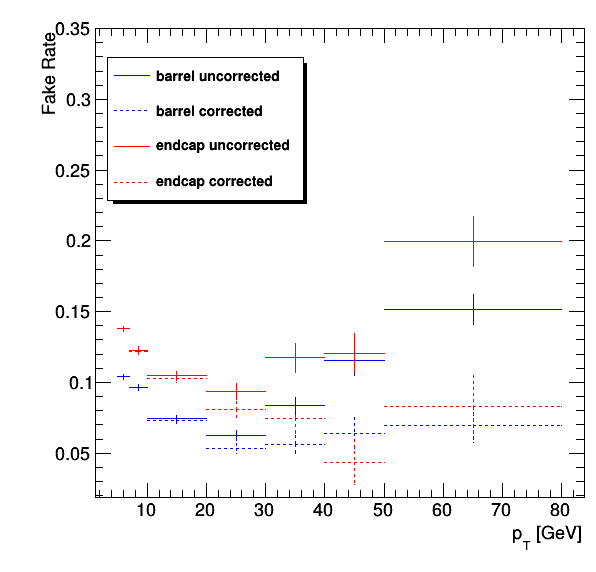
\includegraphics [width=0.45\textwidth] {Figures/RedBkg/FR/FR_OS_muons_2017.png}} \\
    {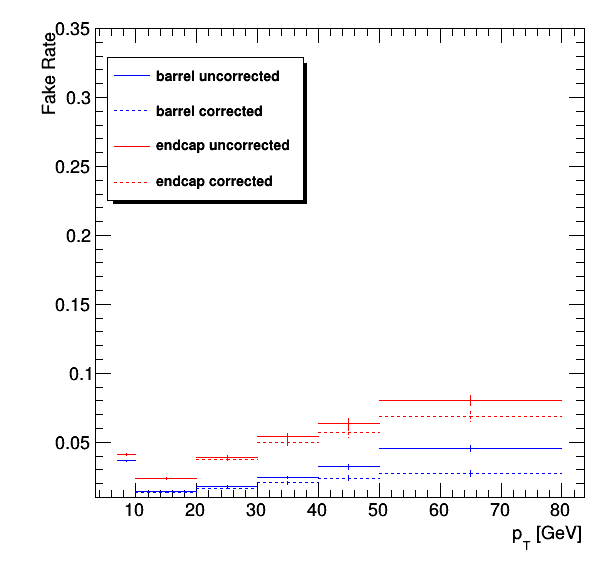
\includegraphics [width=0.45\textwidth] {Figures/RedBkg/FR/FR_OS_electrons_2018.png}}
    {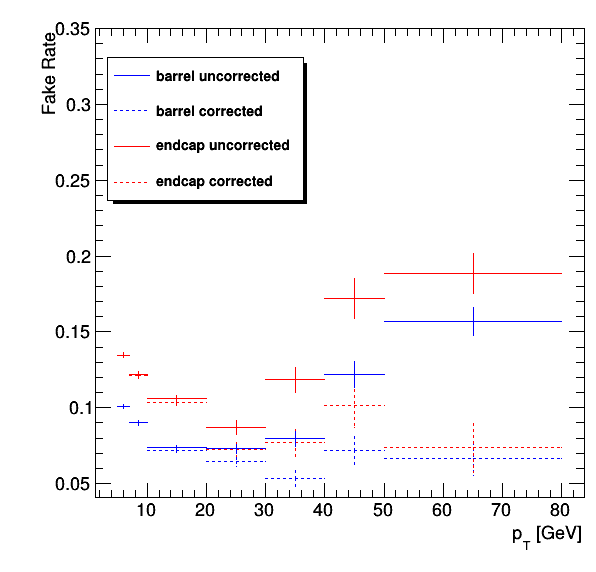
\includegraphics [width=0.45\textwidth] {Figures/RedBkg/FR/FR_OS_muons_2018.png}} 
\caption{
Fake rates as a function of the probe $p_T$ for  electrons (left) and muons (right) which satisfy the loose selection criteria, measured in
a $Z(\ell\ell)+\ell$ sample in the 2016 (top), 2017 (middle) and 2018 (bottom) data at $13$~TeV.
The barrel selection includes electrons (muons) up to $|\eta|$ = 1.479 (1.2). The fake rates are shown before (dotted lines) and after (plain line) removal of WZ contribution from MC.
}
\label{fig:os_fakerates}
\end{center}
\end{figure}
%=======  
The other three leptons should pass the final selection criteria. 

It is expected to be populated with the type of events that populate the
2P+2F region, albeit with different relative proportions,
as well as with $WZ$ events that intrinsically have three prompt leptons.

The control samples obtained in this way, orthogonal by construction
to the signal region, are enriched with fake leptons and are used to
estimate the reducible background in the signal region. 
The invariant mass distribution of events selected in the 2P+2F control sample
is shown in Figures~\ref{fig:2P2F_dataMC2016},~\ref{fig:2P2F_dataMC2017} and~\ref{fig:2P2F_dataMC2018}. 
\begin{figure}[!htb]
\begin{center}
        \subfigure[]{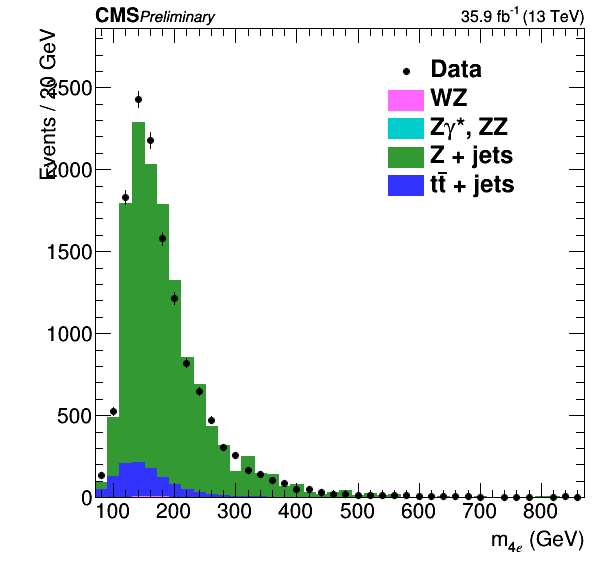
\includegraphics[width=0.45\textwidth]{Figures/RedBkg/M4l_dataMC/M4l_OS_2P2F_4e_2016_Inclusive.png}}
        \subfigure[]{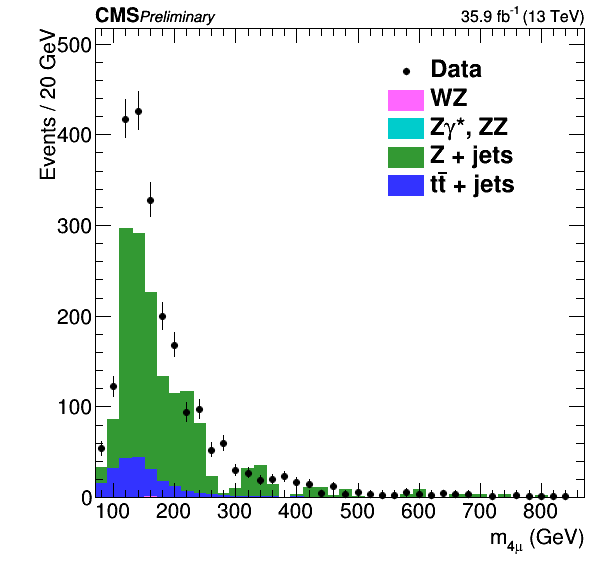
\includegraphics[width=0.45\textwidth]{Figures/RedBkg/M4l_dataMC/M4l_OS_2P2F_4mu_2016_Inclusive.png}}  \\
        \subfigure[]{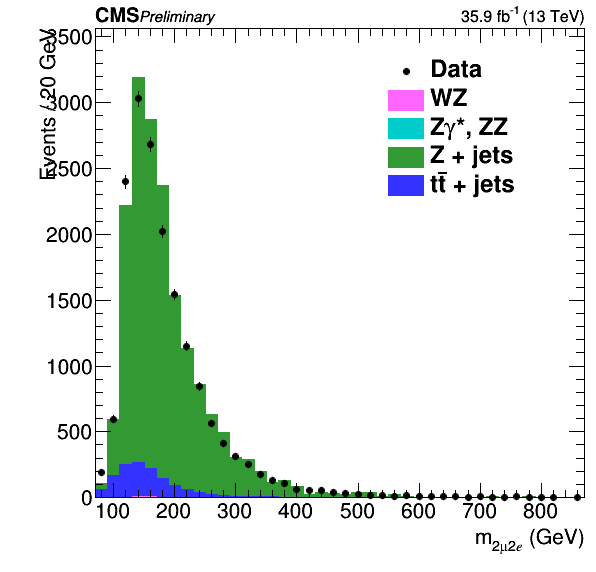
\includegraphics[width=0.45\textwidth]{Figures/RedBkg/M4l_dataMC/M4l_OS_2P2F_2mu2e_2016_Inclusive.png}}
        \subfigure[]{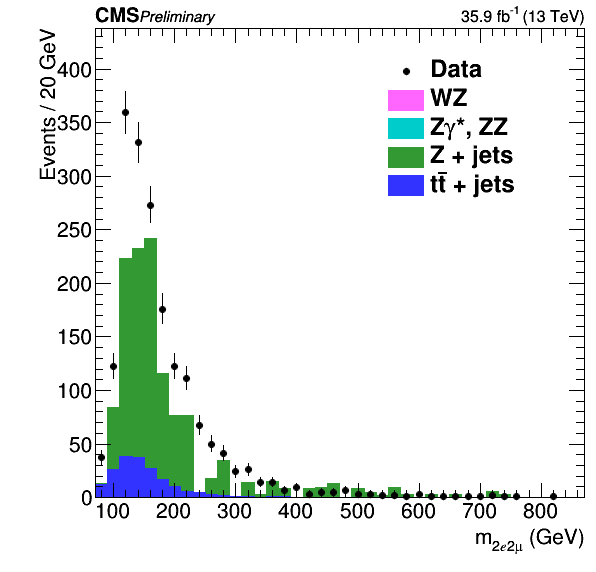
\includegraphics[width=0.45\textwidth]{Figures/RedBkg/M4l_dataMC/M4l_OS_2P2F_2e2mu_2016_Inclusive.png}} \\
\caption{
Invariant mass distribution of the events selected in the 2P+2F control sample in the
2016 dataset for all the considered channels: $4e$ (a), $4\mu$ (b), $2\mu2e$ (c) and $2e2\mu$ (d).
}
\label{fig:2P2F_dataMC2016}
\end{center}
\end{figure}

\begin{figure}[!htb]
\begin{center}
        \subfigure[]{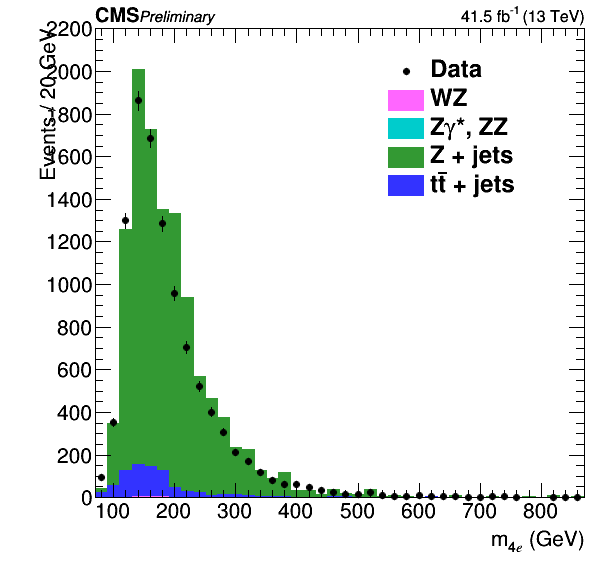
\includegraphics[width=0.45\textwidth]{Figures/RedBkg/M4l_dataMC/M4l_OS_2P2F_4e_2017_Inclusive.png}}
        \subfigure[]{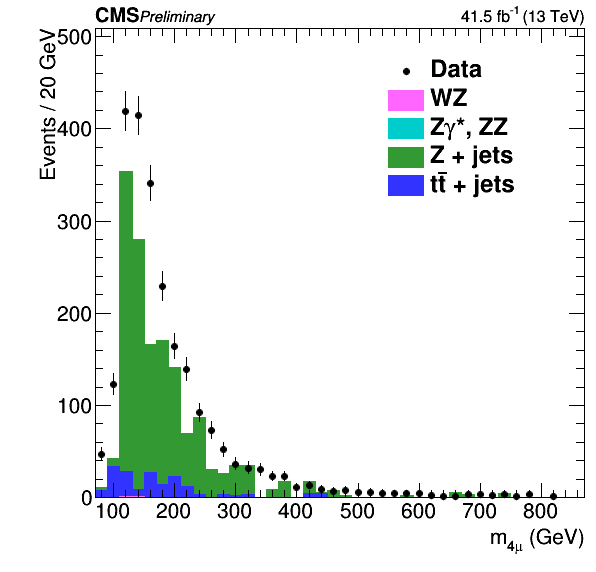
\includegraphics[width=0.45\textwidth]{Figures/RedBkg/M4l_dataMC/M4l_OS_2P2F_4mu_2017_Inclusive.png}}  \\
        \subfigure[]{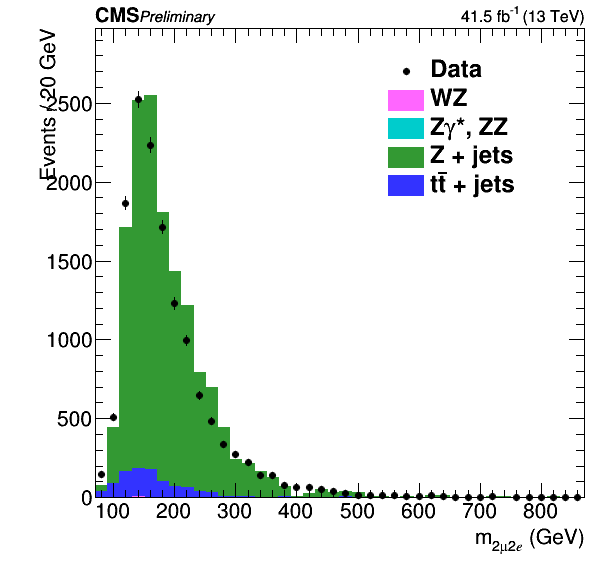
\includegraphics[width=0.45\textwidth]{Figures/RedBkg/M4l_dataMC/M4l_OS_2P2F_2mu2e_2017_Inclusive.png}}
        \subfigure[]{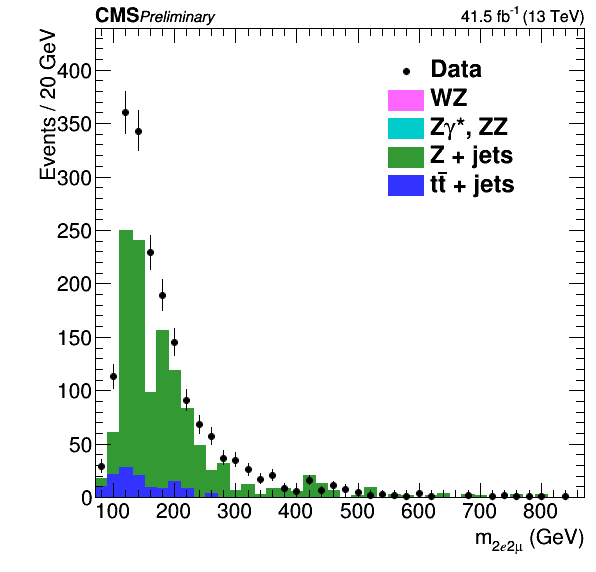
\includegraphics[width=0.45\textwidth]{Figures/RedBkg/M4l_dataMC/M4l_OS_2P2F_2e2mu_2017_Inclusive.png}} \\
\caption{
Invariant mass distribution of the events selected in the 2P+2F control sample in the
2017 dataset for all the considered channels: $4e$ (a), $4\mu$ (b), $2\mu2e$ (c) and $2e2\mu$ (d).
}
\label{fig:2P2F_dataMC2017}
\end{center}
\end{figure}

\begin{figure}[!htb]
\begin{center}
        \subfigure[]{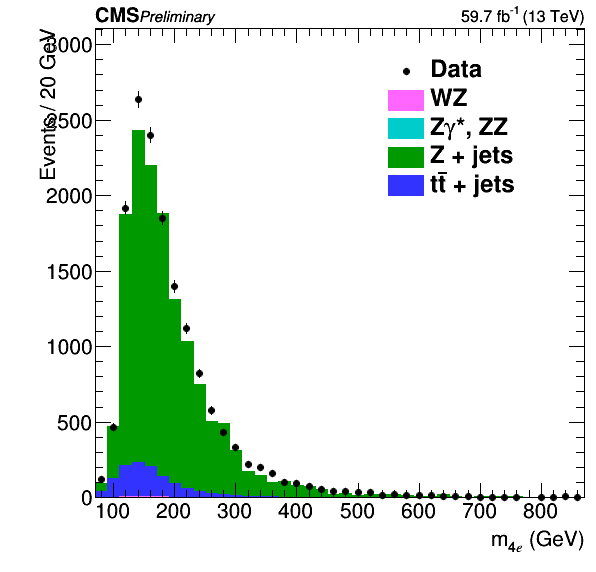
\includegraphics[width=0.45\textwidth]{Figures/RedBkg/M4l_dataMC/M4l_OS_2P2F_4e_2018_Inclusive.png}}
        \subfigure[]{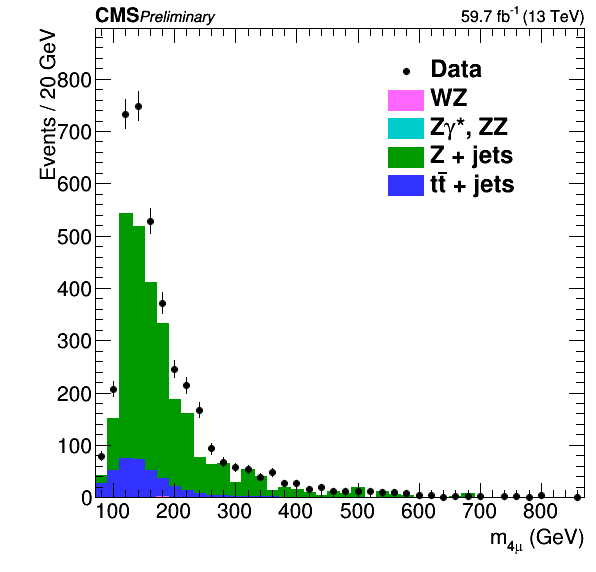
\includegraphics[width=0.45\textwidth]{Figures/RedBkg/M4l_dataMC/M4l_OS_2P2F_4mu_2018_Inclusive.png}}  \\
        \subfigure[]{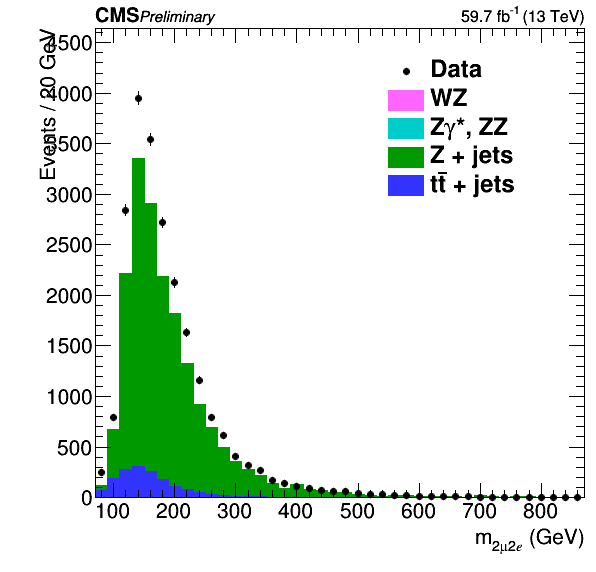
\includegraphics[width=0.45\textwidth]{Figures/RedBkg/M4l_dataMC/M4l_OS_2P2F_2mu2e_2018_Inclusive.png}}
        \subfigure[]{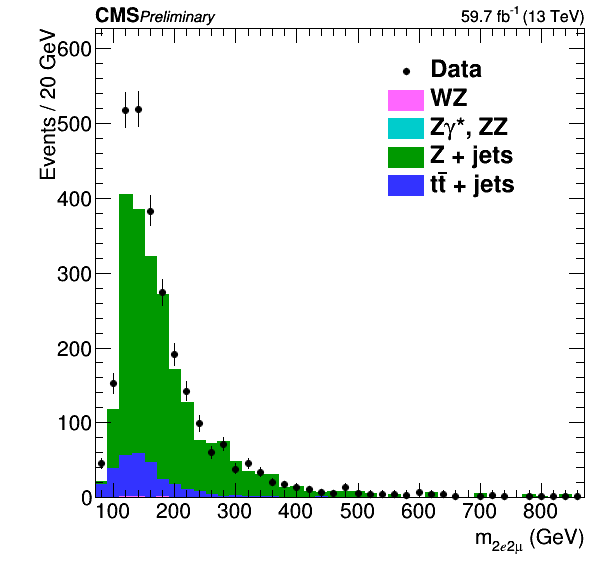
\includegraphics[width=0.45\textwidth]{Figures/RedBkg/M4l_dataMC/M4l_OS_2P2F_2e2mu_2018_Inclusive.png}} \\
\caption{
Invariant mass distribution of the events selected in the 2P+2F control sample in the
2018 dataset for all the considered channels: $4e$ (a), $4\mu$ (b), $2\mu2e$ (c) and $2e2\mu$ (d).
}
\label{fig:2P2F_dataMC2018}
\end{center}
\end{figure}


\begin{figure}[!htb]
\begin{center} 
        \subfigure[]{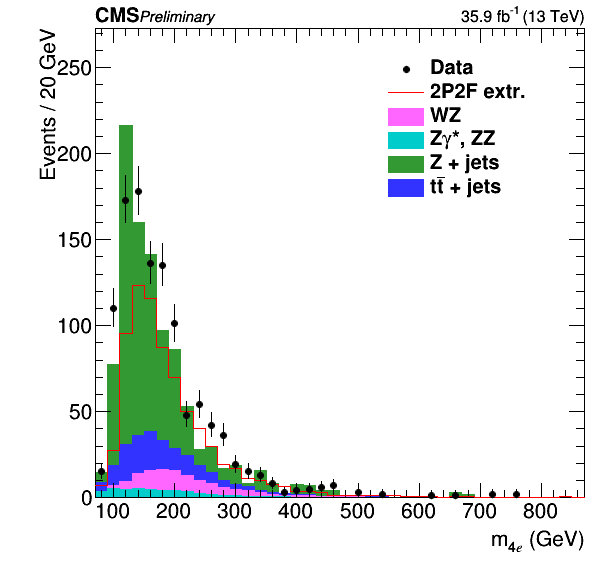
\includegraphics[width=0.45\textwidth]{Figures/RedBkg/M4l_dataMC/M4l_OS_3P1F_4e_2016_Inclusive.png}}
        \subfigure[]{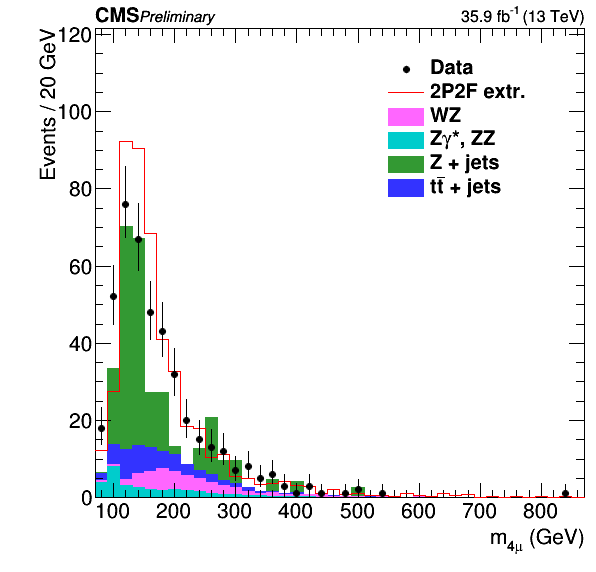
\includegraphics[width=0.45\textwidth]{Figures/RedBkg/M4l_dataMC/M4l_OS_3P1F_4mu_2016_Inclusive.png}}  \\
        \subfigure[]{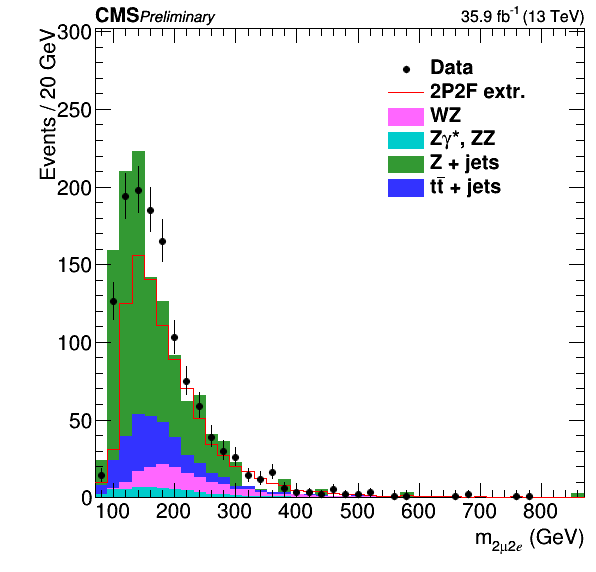
\includegraphics[width=0.45\textwidth]{Figures/RedBkg/M4l_dataMC/M4l_OS_3P1F_2mu2e_2016_Inclusive.png}}
        \subfigure[]{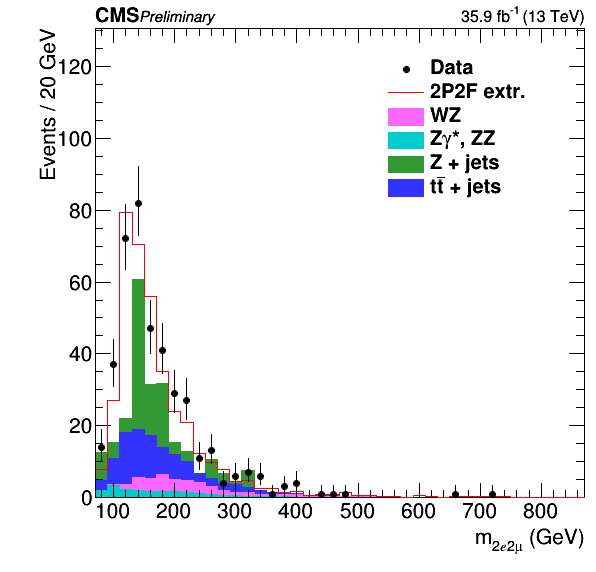
\includegraphics[width=0.45\textwidth]{Figures/RedBkg/M4l_dataMC/M4l_OS_3P1F_2e2mu_2016_Inclusive.png}} \\       
\caption{
Invariant mass distribution of the events selected in the 3P+1F control sample in the
2016 dataset for all the considered channels: $4e$ (a), $4\mu$ (b), $2\mu2e$ (c) and $2e2\mu$ (d).
}
\label{fig:CR_3P1F2016}
\end{center}
\end{figure}

\begin{figure}[!htb]
\begin{center} 
        \subfigure[]{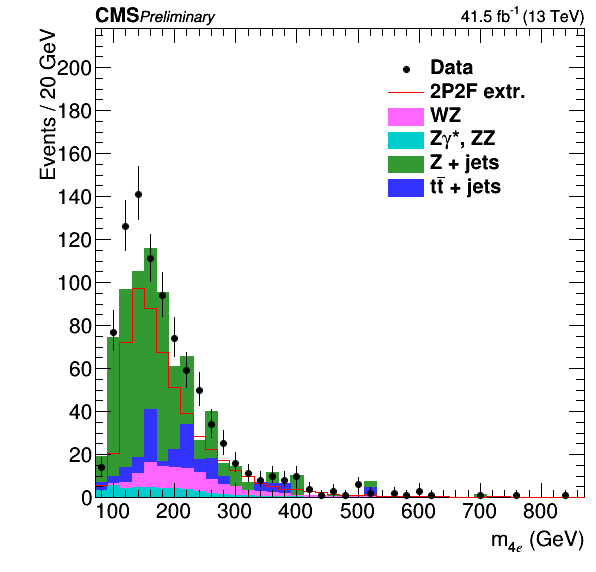
\includegraphics[width=0.45\textwidth]{Figures/RedBkg/M4l_dataMC/M4l_OS_3P1F_4e_2017_Inclusive.png}}
        \subfigure[]{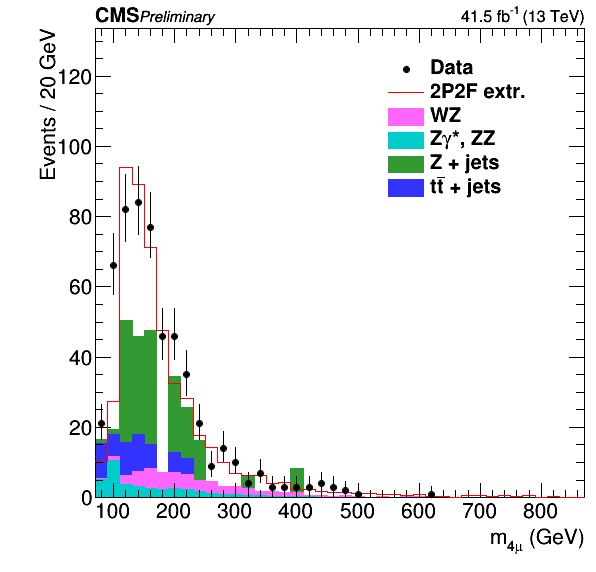
\includegraphics[width=0.45\textwidth]{Figures/RedBkg/M4l_dataMC/M4l_OS_3P1F_4mu_2017_Inclusive.png}}  \\
        \subfigure[]{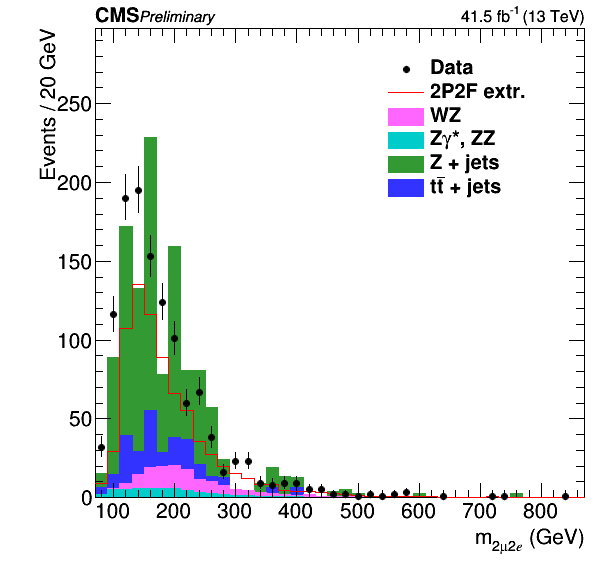
\includegraphics[width=0.45\textwidth]{Figures/RedBkg/M4l_dataMC/M4l_OS_3P1F_2mu2e_2017_Inclusive.png}}
        \subfigure[]{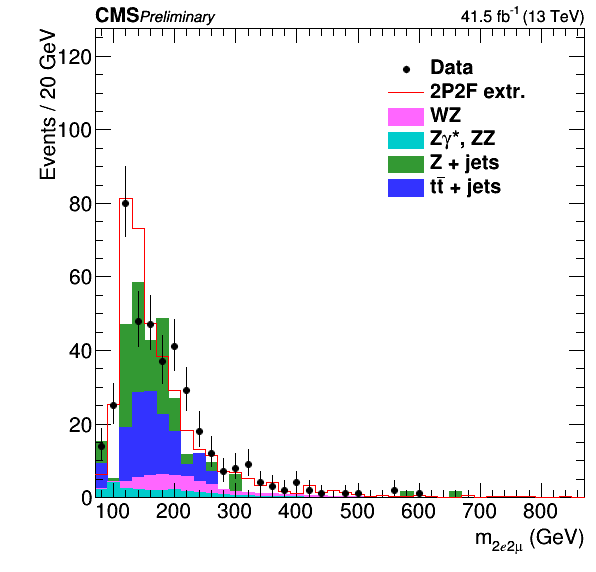
\includegraphics[width=0.45\textwidth]{Figures/RedBkg/M4l_dataMC/M4l_OS_3P1F_2e2mu_2017_Inclusive.png}} \\       
\caption{
Invariant mass distribution of the events selected in the 3P+1F control sample in the
2017 dataset for all the considered channels: $4e$ (a), $4\mu$ (b), $2\mu2e$ (c) and $2e2\mu$ (d).
}
\label{fig:CR_3P1F2017}
\end{center}
\end{figure}

\begin{figure}[!htb]
\begin{center} 
        \subfigure[]{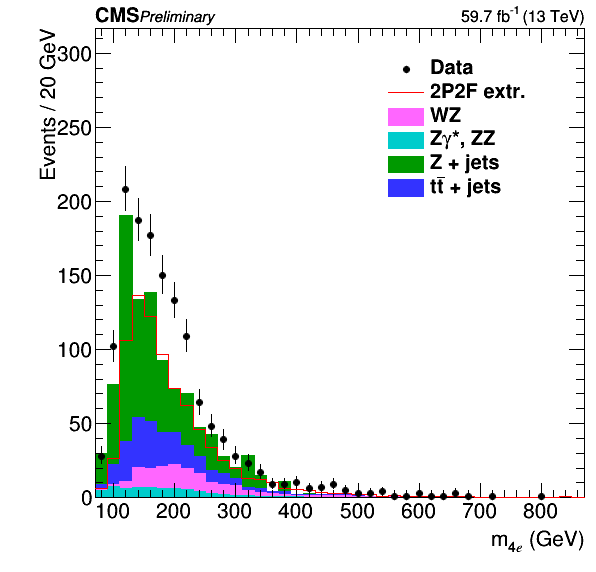
\includegraphics[width=0.45\textwidth]{Figures/RedBkg/M4l_dataMC/M4l_OS_3P1F_4e_2018_Inclusive.png}}
        \subfigure[]{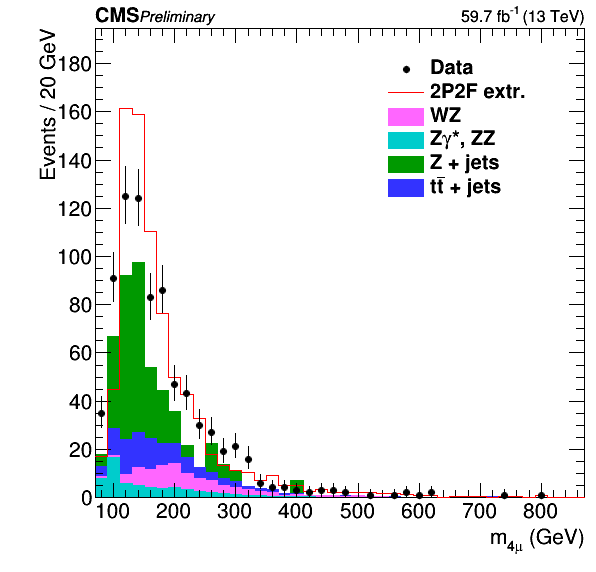
\includegraphics[width=0.45\textwidth]{Figures/RedBkg/M4l_dataMC/M4l_OS_3P1F_4mu_2018_Inclusive.png}}  \\
        \subfigure[]{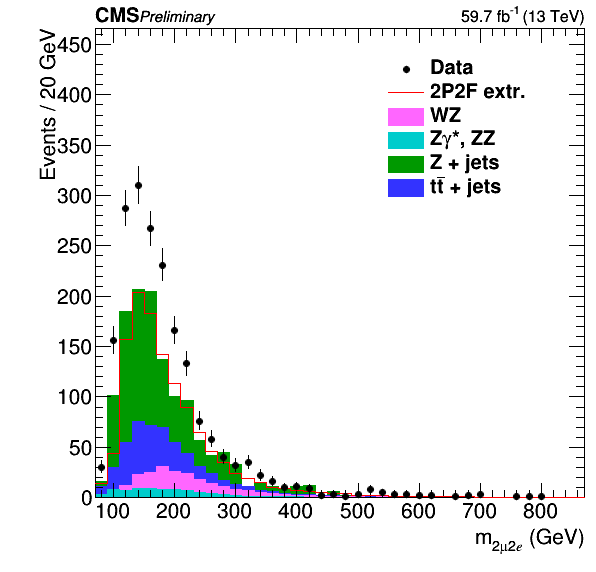
\includegraphics[width=0.45\textwidth]{Figures/RedBkg/M4l_dataMC/M4l_OS_3P1F_2mu2e_2018_Inclusive.png}}
        \subfigure[]{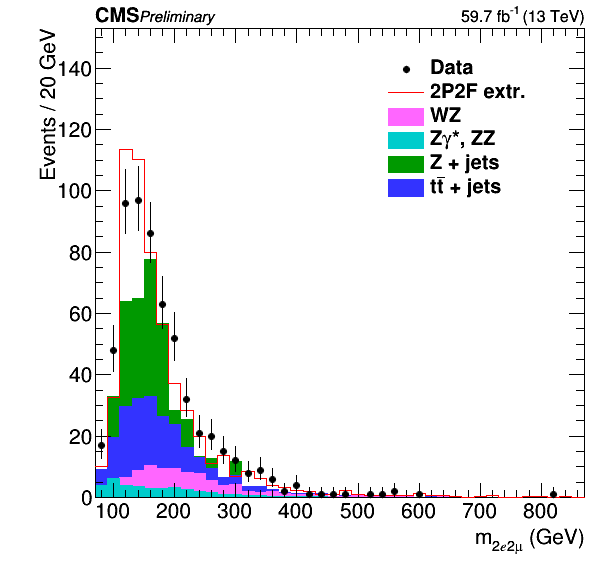
\includegraphics[width=0.45\textwidth]{Figures/RedBkg/M4l_dataMC/M4l_OS_3P1F_2e2mu_2018_Inclusive.png}} \\       
\caption{
Invariant mass distribution of the events selected in the 3P+1F control sample in the
2018 dataset for all the considered channels: $4e$ (a), $4\mu$ (b), $2\mu2e$ (c) and $2e2\mu$ (d).
}
\label{fig:CR_3P1F2018}
\end{center}
\end{figure}

The expected number of reducible background events in the 3P+1F region,
$N^{\rm bkg}_{\rm 3P1F}$, can be computed from the number of events
observed in the 2P+2F control region, $N_{\rm 2P2F}$, by weighting each
event in the region with the factor $(\frac{f_{i}}{1-f_{i}}
+ \frac{f_{j}}{1-f_{j}})$, where $f_{i}$ and $f_{j}$ correspond to the
fake ratios of the two loose leptons:

\begin{equation} 
\label{eq:Prediction3P1F}
N^{\rm bkg}_{\rm 3P1F} = \sum (\frac{f_{i}}{1-f_{i}}
+ \frac{f_{j}}{1-f_{j}}) N_{\rm 2P2F}
\end{equation} 

Figures~\ref{fig:CR_3P1F2016},~\ref{fig:CR_3P1F2017} and~\ref{fig:CR_3P1F2018} shows the invariant mass distributions of the
events selected in the 3P+1F control sample, together with the expected
reducible background estimated from Eq.~\ref{eq:Prediction3P1F},
stacked on the distribution
of $WZ$ and of irreducible background ($ZZ, Z\gamma* \to 4\ell$) taken from the simulation.

Would the fake rates be measured in a sample that has exactly the same
background composition as the 2P+2F sample, the difference between the
observed number of events in the 3P+1F sample and the expected background
predicted from the 2P+2F sample would solely amount to the (small) $WZ$ and $Z\gamma_{conv}$
contribution. Large differences arise because the fake rates used in
Eq.~\ref{eq:Prediction3P1F} do not properly account for the background
composition of the 2P+2F control sample.


In particular, the  difference seen in Figure~\ref{fig:CR_3P1F2018} between the observed
3P+1F distribution and the expectation from 2P+2F, in the
channels with loose electrons ($4e$ and $2\mu2e$), and concentrated at low
masses, is due to photon conversions. This is confirmed explicitly by the
simulation.
% : Figure~\ref{fig:CR_3P1F}c shows how events with a real photon populate
% this low mass region. Indeed, as the fake rates of method A are measured
% in a sample that is largely devoid of photon conversions, Eq.~\ref{eq:Prediction3P1F}
% considerably underestimates their contribution to the 3P+1F sample. 
%
The difference between the 3P+1F observation and the prediction
from 2P+2F to recover the missing contribution from conversions - and more generally,
in principle, to ``correct" for the fact that the fake rates do not properly
account for the background composition of the 2P+2F sample.
More precisely, the expected reducible background in the signal region is given
by the sum of two terms :
%
\begin{itemize}
\item a ``2P2F component", obtained from the number of
  events observed in the 2P+2F control region, $N_{\rm 2P2F}$, by
  weighting each event in that region with the factor
  $\frac{f_{i}}{1-f_{i}} \frac{f_{j}}{1-f_{j}}$, where $f_{i}$ and
  $f_{j}$ correspond to the fake ratios of the two loose leptons;
\item a ``3P1F component", obtained from the
   difference between the number of observed events in the 3P+1F control
   region, $N_{\rm 3P1F}$, and the expected contribution from the 2P+2F
   region and ZZ processes in the signal region, $N^{\rm ZZ}_{\rm 3P1F} +
   N^{\rm bkg}_{\rm 3P1F}$. The $N^{\rm bkg}_{\rm 3P1F}$ is given by 
   Eq. \ref{eq:Prediction3P1F} and $N^{\rm ZZ}_{\rm 3P1F}$ is the
   contribution from $ZZ$ which is taken from the simulation. 
   The difference $N_{\rm 3P1F} -  N^{\rm bkg}_{\rm 3P1F} - N^{\rm ZZ}_{\rm 3P1F}$,
   which may be negative,
   is obtained for each $(p_T, \eta)$ bin of the ``F" lepton, and is weighted 
   by $\frac{f_i} {1 - f_i}$, where $f_i$ denotes the fake rate of
   this lepton.
   This ``3P1F component" accounts for the contribution of reducible background
   processes with only one fake lepton (like $WZ$ events), and for the contribution
   of other processes (e.g. photon conversions) that are not properly estimated
   by the 2P2F component, because of the fake rates used.
\end{itemize}

Therefore, the full expression for the prediction can be symbolically written as:
%
\begin{equation} 
\label{eq:PredictionSR}
N^{bkg}_{\rm SR} = \sum \frac{f_{i}}{(1-f_{i})} (N_{\rm 3P1F} - N^{\rm
bkg}_{\rm 3P1F} - N^{\rm ZZ}_{\rm 3P1F})
+ \sum \frac{f_{i}}{(1-f_{i})} \frac{f_{j}}{(1-f_{j})}N_{\rm 2P2F} \end{equation}
%a
Previous equation is equivalent to the following:
\begin{equation}
\label{eq:PredictionSR2}
N^{bkg}_{\rm SR}= (1-\frac{N_{3P1F}^{ZZ}}{N_{3P1F}})\sum_j^{N_{3P1F}}\frac{f_a^j}{1-f_a^j} - \sum_i^{N_{2P2F}}\frac{f_3^i}{1-f_3^i}\frac{f_4^i}{1-f_4^i}
\end{equation}
For channels where the $Z_2$ candidate is made from two electrons, 
the contribution of the 3P1F component is 
positive, and amounts to typically $30 \%$ of the total predicted background.

For channels with loose muons ($4\mu$ and $2e2\mu$), the 3P+1F sample is rather well described by
the prediction from 2P+2F, as seen in Figure~\ref{fig:CR_3P1F2018}, and the
3P1F component is mainly driven by statistical fluctuations in the 3P+1F sample,
which are larger than the expectation from $WZ$ production.


%%%%%%%%%%%%%%%%%%%%%%%
Table~\ref{tab:reducibleMethodA} shows the expected number of
events in the signal regions from the reducible background processes at $13$~TeV for each considered final state and for all three years using the OS method.
%The uncertainty is given by the combination of a statistical uncertainty, which is dominated by the large statistical uncertainty of the ``3P1F" component, 
%and a systematic uncertainty due to the statistical uncertainty of the fake rates.
The invariant mass distribution of the ZX events obtained from the combination of the results in the 2P+2F and 3P+1F control samples
are shown in Figure~\ref{fig:combOS_dataMC2016},~\ref{fig:combOS_dataMC2017},~\ref{fig:combOS_dataMC2018}.
\begin{figure}[!htb]
\begin{center}
        \subfigure[]{\includegraphics[width=0.45\textwidth]{Figures/RedBkg/M4l_dataMC/M4l_OS_4e_2016-Inclusive.png}}
        \subfigure[]{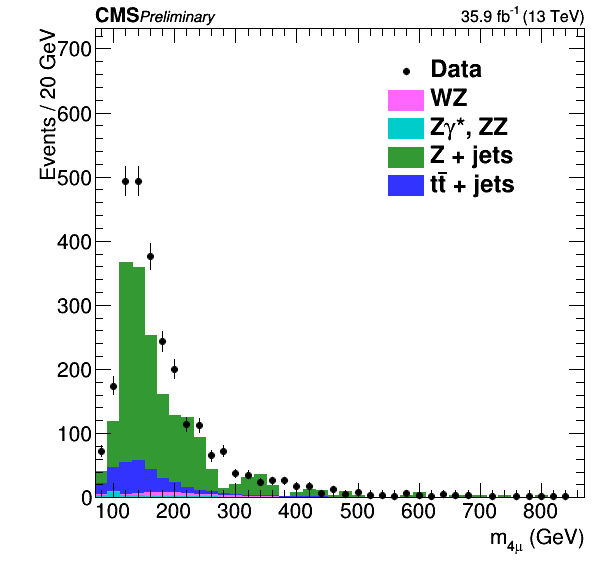
\includegraphics[width=0.45\textwidth]{Figures/RedBkg/M4l_dataMC/M4l_OS_4mu_2016_Inclusive.png}}  \\
        \subfigure[]{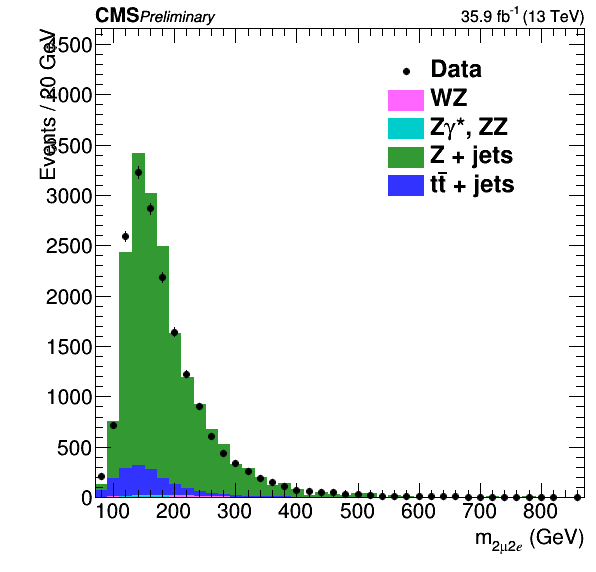
\includegraphics[width=0.45\textwidth]{Figures/RedBkg/M4l_dataMC/M4l_OS_2mu2e_2016_Inclusive.png}}
        \subfigure[]{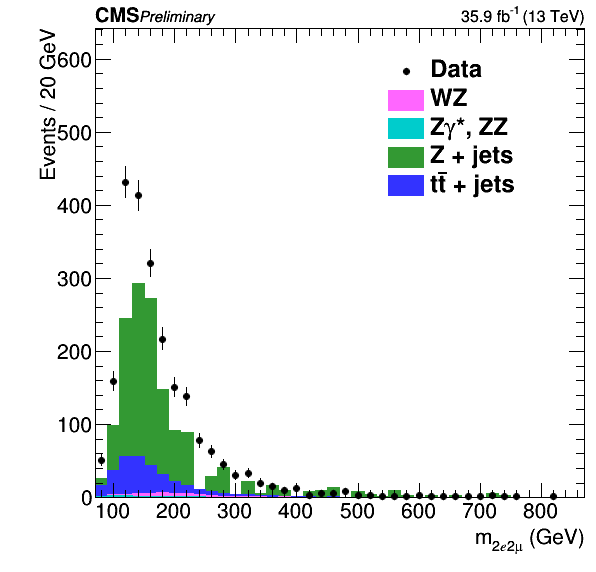
\includegraphics[width=0.45\textwidth]{Figures/RedBkg/M4l_dataMC/M4l_OS_2e2mu_2016_Inclusive.png}} \\       
\caption{
Invariant mass distribution of the events selected in the 2P+2F and 3P+1F control samples in the
2018 dataset for all the considered channels: $4e$ (a), $4\mu$ (b), $2\mu2e$ (c) and $2e2\mu$ (d) for 2016 data.
}
\label{fig:combOS_dataMC2016}
\end{center}
\end{figure}

\begin{figure}[!htb]
\begin{center}
        \subfigure[]{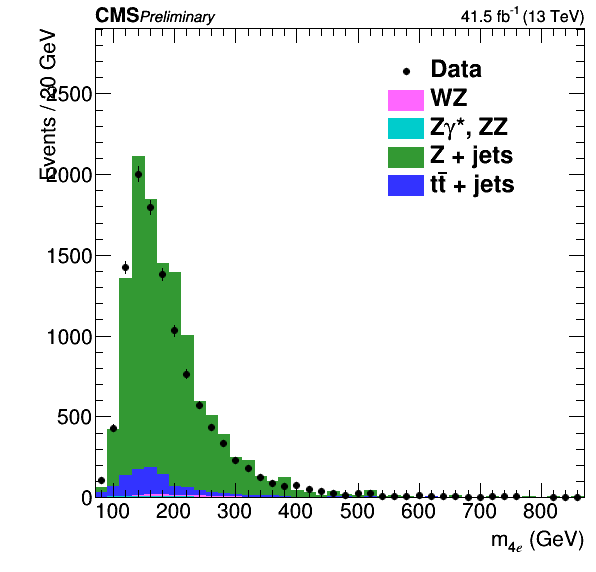
\includegraphics[width=0.45\textwidth]{Figures/RedBkg/M4l_dataMC/M4l_OS_4e_2017_Inclusive.png}}
        \subfigure[]{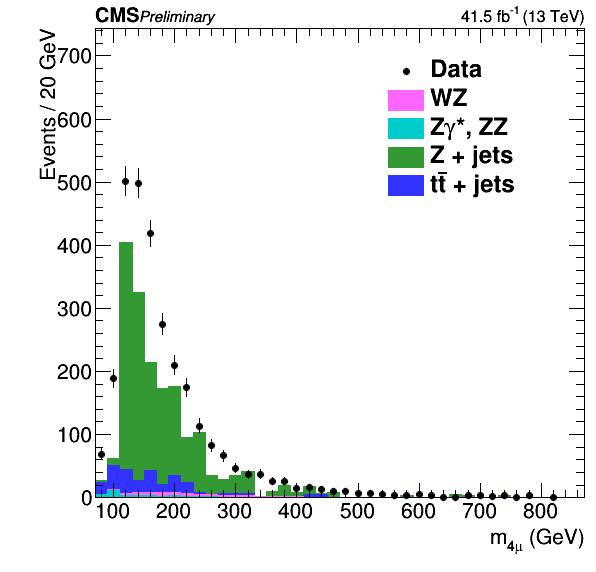
\includegraphics[width=0.45\textwidth]{Figures/RedBkg/M4l_dataMC/M4l_OS_4mu_2017_Inclusive.png}}  \\
        \subfigure[]{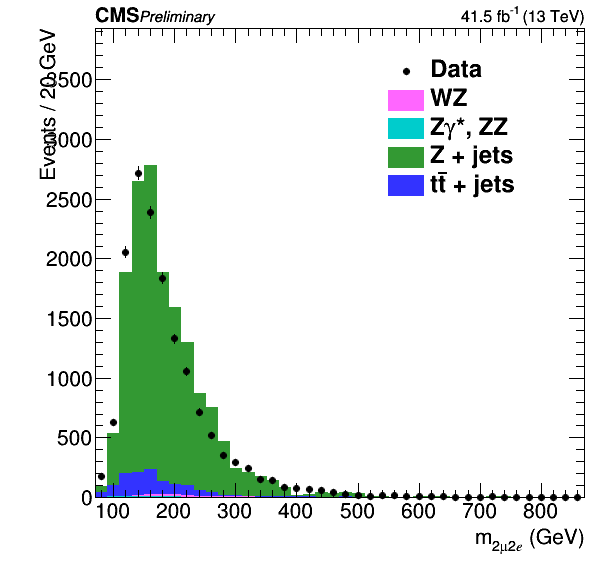
\includegraphics[width=0.45\textwidth]{Figures/RedBkg/M4l_dataMC/M4l_OS_2mu2e_2017_Inclusive.png}}
        \subfigure[]{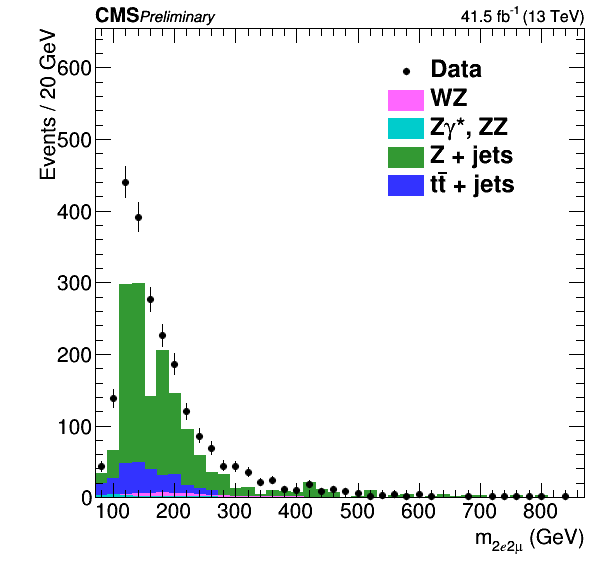
\includegraphics[width=0.45\textwidth]{Figures/RedBkg/M4l_dataMC/M4l_OS_2e2mu_2017_Inclusive.png}} \\       
\caption{
Invariant mass distribution of the events selected in the 2P+2F and 3P+1F control samples in the
2018 dataset for all the considered channels: $4e$ (a), $4\mu$ (b), $2\mu2e$ (c) and $2e2\mu$ (d) for 2017 data.
}
\label{fig:combOS_dataMC2017}
\end{center}
\end{figure}

\begin{figure}[!htb]
\begin{center}
        \subfigure[]{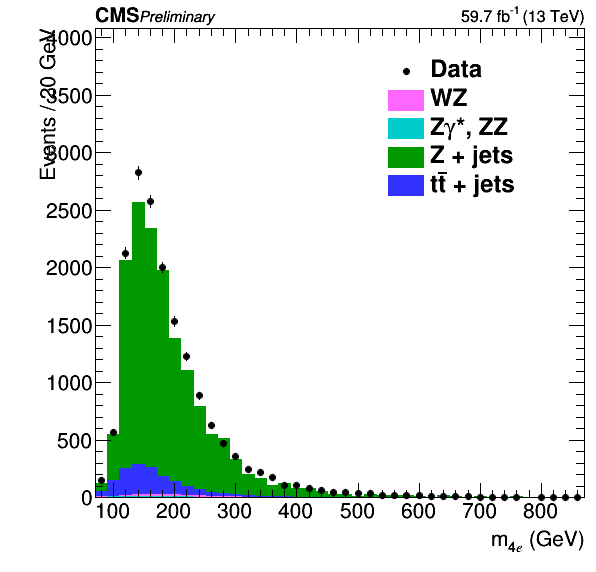
\includegraphics[width=0.45\textwidth]{Figures/RedBkg/M4l_dataMC/M4l_OS_4e_2018_Inclusive.png}}
        \subfigure[]{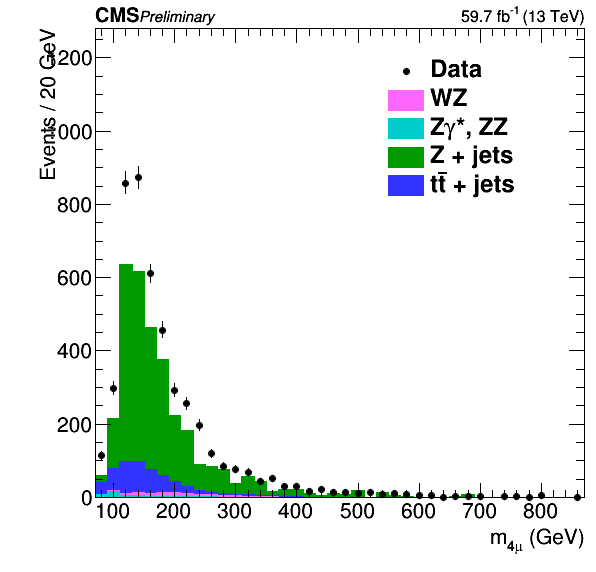
\includegraphics[width=0.45\textwidth]{Figures/RedBkg/M4l_dataMC/M4l_OS_4mu_2018_Inclusive.png}}  \\
        \subfigure[]{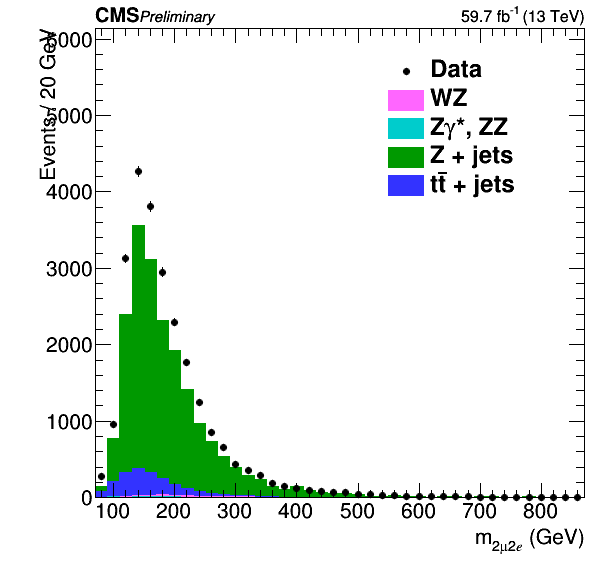
\includegraphics[width=0.45\textwidth]{Figures/RedBkg/M4l_dataMC/M4l_OS_2mu2e_2018_Inclusive.png}}
        \subfigure[]{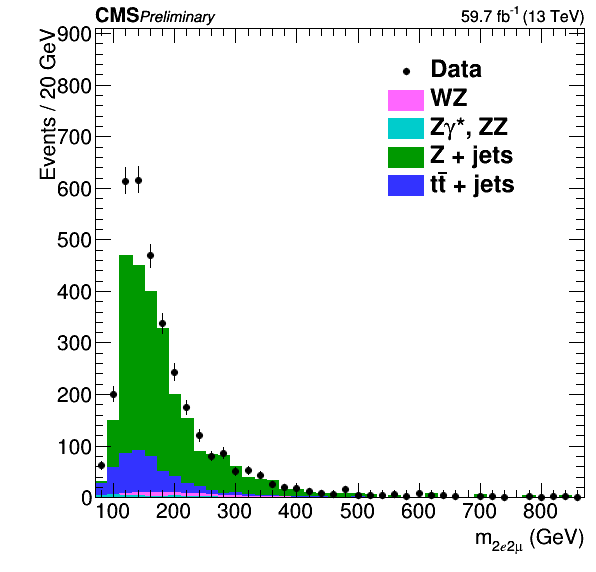
\includegraphics[width=0.45\textwidth]{Figures/RedBkg/M4l_dataMC/M4l_OS_2e2mu_2018_Inclusive.png}} \\       
\caption{
Invariant mass distribution of the events selected in the 2P+2F and 3P+1F control samples in the
2018 dataset for all the considered channels: $4e$ (a), $4\mu$ (b), $2\mu2e$ (c) and $2e2\mu$ (d) for 2018 data.
}
\label{fig:combOS_dataMC2018}
\end{center}
\end{figure}



\begin{table}[h]
\begin{center}
     \begin{tabular}{| l | c | c | c | c |} \hline
Channel	& 4e 	           & 4$\mu$          & 2e2$\mu$        & 2$\mu$2e        \\ \hline \hline
2016    & $ 20.1 \pm 6.1 $ & $26.9 \pm 8.6$ & $25.2 \pm 8.0$  & $22.3 \pm 6.8$  \\ 
2017    & $ 16.2 \pm 5.0 $ & $32.7 \pm 10.3$ & $24.0 \pm 7.7$  & $21.3 \pm 6.5$  \\ 
2018    & $ 25.4 \pm 7.7 $ & $49.4 \pm 15.4$ & $34.2 \pm 10.7$ & $33.0 \pm 10.0$ \\ \hline 
 	\end{tabular}
\end{center}
    \caption{ The contribution of reducible background
    processes in the signal region predicted from measurements in 2016, 2017 and 2018 data
    using the OS method. The predictions correspond to 35.9, 41.5 and 59.7~fb$^{-1}$ of data at $13$~TeV, respectively.}
     \label{tab:reducibleMethodA}
\end{table}
